\documentclass[a4paper,norsk]{article}
\usepackage{preamble}
\graphicspath{ {Circle}{ellipse} }


\begin{document}

\title{Marine Hydrodynamics \\ Assignment 1}
\author{Sebastian Gjertsen}

\maketitle
\begin{center}
\subsection*{Assignment}

For specified (see below) two-dimensional geometries, assuming potential theory in unbounded fluid, and use of Green's second identity, calculate the velocity potential along the body and the added mass forces, for a circle, an ellipse, a square and a rectangle, moving laterally, and with rotation. Find also the cross coupling added mass coefficients. For the circle, the reference solution is: $ \phi =-a^2/(x^2)$ where a denotes the cylinder radius, $r^2=x^2+y^2$.
\end{center}


\section*{Theory, numerics and program}
In this assignment we use the method of panels. By splitting the geometry into N equal parts, and assuming that $\phi , \frac{\partial \phi }{\partial n}$ is constant every segment.
\newline
From Newman chapter 4 we have (79):
\[   \int_C \phi \frac{\partial G }{\partial n} - G\frac{\partial \phi }{\partial n} = -\pi \phi(x,y) \]
where $G = ln (r)$, a source in 2D, and C is the circumference of the geometry
$$ -\pi \phi(x_0) + \int_C \phi \frac{\partial }{\partial n} ln(r) dl = \int_C ln(r) \frac{\partial \phi}{\partial n} dl       $$
where $x_0$ states a point on our geometry.\\
\newline
We got a trick from the lectures, turning it into:
\[ -\pi phi(x_0) + \sum_{n=1}^N \phi(x_n) (\theta_a - \theta_b)  = \int_C ln(r)\frac{\partial \phi }{\partial n} dl    \]
$$
\begin{pmatrix}
  -\pi & (\theta_a - \theta_b)_0  & (\theta_a - \theta_b)_1 & ...\\
  (\theta_a - \theta_b)_N  & -\pi & (\theta_a - \theta_b)_0  & ...\\
  (\theta_a - \theta_b)_{N-1}  & (\theta_a - \theta_b)_N  & -\pi & ...\\
  ... & ... & ....& ...  \\
 \end{pmatrix}
 \begin{pmatrix}
\phi_0  \\
\phi_1 \\
\phi_2 \\ 
  ...  \\
  \phi_N
 \end{pmatrix}
 =
 \begin{pmatrix}
\int ln(r_0)\frac{\partial \phi }{\partial n} dl   \\
\int ln(r_1)\frac{\partial \phi }{\partial n} dl  \\
\int ln(r_2)\frac{\partial \phi }{\partial n} dl  \\ 
  ...  \\
  \end{pmatrix}
  $$
To calculate the $\phi$ values we created a fictional point between the $x_N$ points, where we stand in this "ghost" point and calculate the $\Delta \theta$ to the $x_N$ values. This is done since we have assumed $\phi$ to be constant.
To evaluate the integrals we used the trapezoidal method.
Every line of the matrix on the right hand side is calculated by going around the geometry once.

The normal vector is defined as:

$$\bar{n} = \frac{\frac{x}{a^2}\bar{i} + \frac{y}{b^2}\bar{j} } { (\frac{x}{a^2})^2 + (\frac{y}{b^2})^2 }$$
which is used for ellipse and for circle when $a=b$.

For a circle we have an exact solution for $\phi =-\frac{a^2x}{r^2} $, which is $\phi = -a cos(\theta)$ and an exact solution for added mass $m_{11} = \rho r_a^2 \pi $
\newline
For an ellipse we only have the exact solution for added mass $m_{11} = \rho r_a^2 \pi$, $   m_{22} = \rho r_b^2 \pi $,   $m{66} = \frac{\pi}{8}\rho(r_a^2-r_b^2)^2 $.
\newline
Next page is the program code in Python
\newpage
\lstinputlisting[style= python]{Oblig1.py}
\newpage

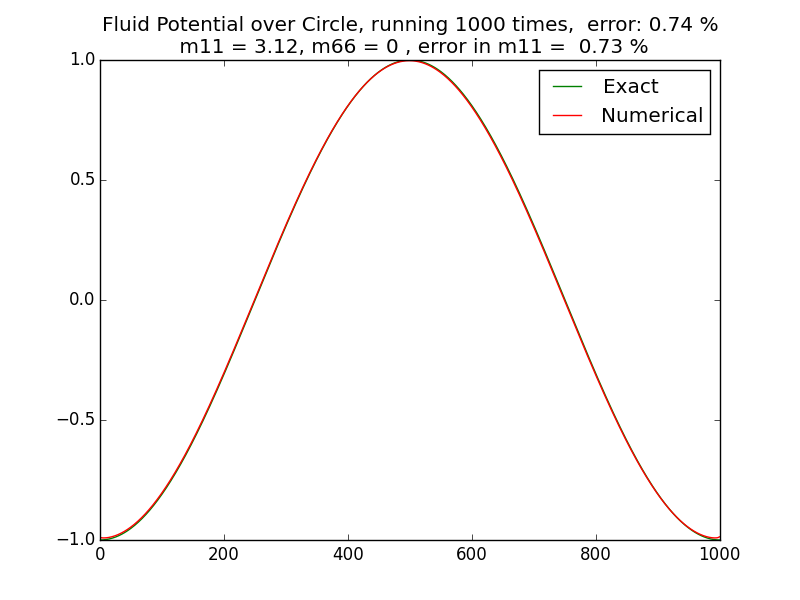
\includegraphics[width=13cm, height=10cm]{Circle}
\newline
This shows a plot of $\phi$ over a circle, with the added mass and errors calculated.
\newline
We can see that the error of $\phi$ compared to the exact solution is $0.74  \%$ 
and the added mass $m_{66}$ has an error of $0.73 \% $ . The added mass $m_{66}$ is of course zero because we have a circle.
With these small error i am convinced that the program works for a circle. Next up an ellipse:
\newpage
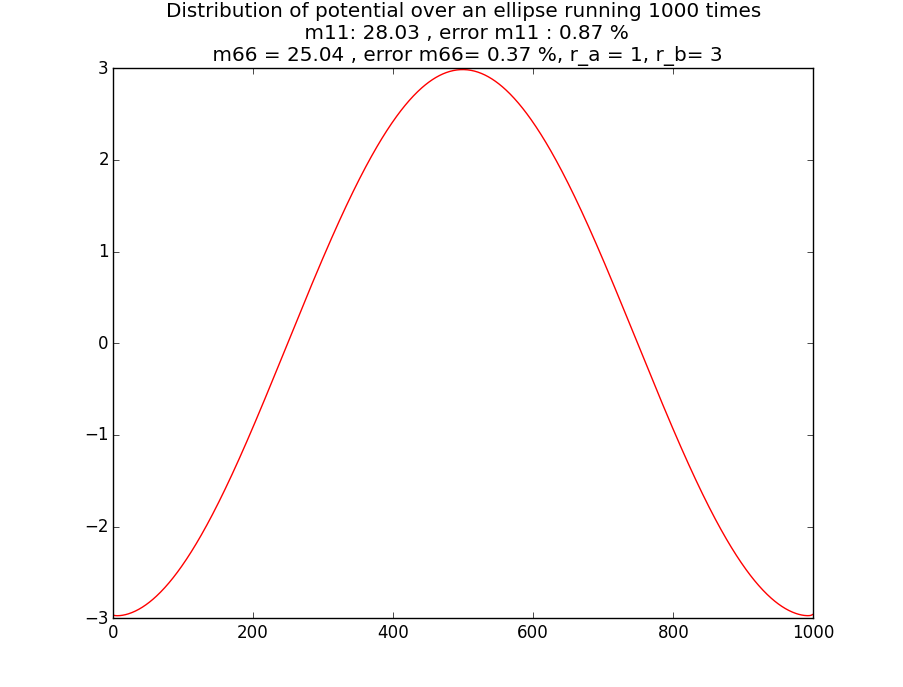
\includegraphics[width=13cm, height=10cm]{ellipse}
\newline
This plot is over an ellipse. Again we can see that the errors are very small $0.87 \% $  and $0.37\%$
With both of our geometries having so small error compared to the analytics, I am convinced that the program is correct and the potential and added masses are correctly calculated.
I have not calculated the added mass $m_{22}, m_{12}, m_{21}$ as these will all be zero since the geometry only travels laterally.
\newline
Since i am not very good in Latex , the code does not look very good copied in. Please let me know if you want the Python code.







\end{document}